
\begin{figure}
    \centering
    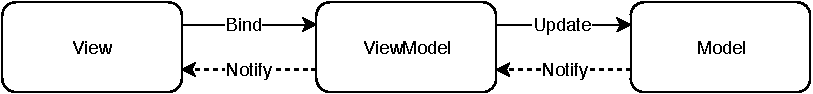
\includegraphics[scale=0.7]{images/MVVM.pdf}
    \caption{Entity Relationship Diagram}
    \label{fig:mvvm}
\end{figure}

The architectural pattern principle enhances the separation of \textit{graphical user interface} logic from the \textit{oparting system} interactions \cite{architecture}. The Model-View-ViewModel (hereafter: MVVM) is an architectural pattern which is well-integrated and incentived by Android. It has three components that consititute the principle:
\begin{itemize}
    \item \verb|Model|: represents the data and the business logic of the application. 
    \item \verb|ViewModel|: interacts with the model, and manages the state of the view.
    \item \verb|View|: handles and manages the user interface of the application.
\end{itemize}

In Figure \ref{fig:mvvm}, the interactions amongst the components are illustrated. The connection between the \verb|View| and \verb|ViewModel| occurs over a data binding connection, which enables the view to change automatically based on changes to the binding of the subscribed data \cite{mvvm}. In Android, the \verb|LiveData| is an obserable data holder that enables data binding, which allows components to observe for data changes. \verb|LiveData| respects the lifecycle of the application components (e.g., activities, fragments, or services), ensuring the \verb|LiveData| only updates the components that are in an active lifecycle state \cite{livedata}. Moreover, \verb|Android Room| provides set of components to facilitate the structure of the model component \cite{room}. More spesifically, it models a database and the entities (which are the tables in the database). In our application, we use this architectural pattern to interact and to model for our data entities (see Section X). 


